\documentclass[conf]{new-aiaa}
%\documentclass[journal]{new-aiaa} for journal papers
\usepackage[utf8]{inputenc}

\usepackage{graphicx}
\usepackage{amsmath}
\usepackage[version=4]{mhchem}
\usepackage{listings}
\usepackage{color}
\usepackage{siunitx}
\usepackage{longtable,tabularx}
\usepackage{subcaption}
\usepackage{cleveref}
\usepackage{appendix}
\setlength\LTleft{0pt}

\title{Laminar viscous supersonic flow over flat plate}

\author{Ramkumar S.}
% \affil{SC22M007, M.Tech. Aerospace - Aerodynamics and Flight Mechanics}


\definecolor{mygreen}{rgb}{0,0.6,0}
\definecolor{mygray}{rgb}{0.5,0.5,0.5}
\definecolor{mymauve}{rgb}{0.58,0,0.82}

\lstset{
  backgroundcolor=\color{white},   % choose the background color; you must add \usepackage{color} or \usepackage{xcolor}; should come as last argument
  basicstyle=\footnotesize,        % the size of the fonts that are used for the code
  breakatwhitespace=false,         % sets if automatic breaks should only happen at whitespace
  breaklines=true,                 % sets automatic line breaking
  captionpos=b,                    % sets the caption-position to bottom
  commentstyle=\color{mygreen},    % comment style
  deletekeywords={...},            % if you want to delete keywords from the given language
  escapeinside={\%*}{*)},          % if you want to add LaTeX within your code
  extendedchars=true,              % lets you use non-ASCII characters; for 8-bits encodings only, does not work with UTF-8
  firstnumber=0001,                % start line enumeration with line 1000
  frame=single,                    % adds a frame around the code
  keepspaces=true,                 % keeps spaces in text, useful for keeping indentation of code (possibly needs columns=flexible)
  keywordstyle=\color{blue},       % keyword style
  language=Octave,                 % the language of the code
  morekeywords={*,...},            % if you want to add more keywords to the set
  numbers=left,                    % where to put the line-numbers; possible values are (none, left, right)
  numbersep=5pt,                   % how far the line-numbers are from the code
  numberstyle=\tiny\color{mygray}, % the style that is used for the line-numbers
  rulecolor=\color{black},         % if not set, the frame-color may be changed on line-breaks within not-black text (e.g. comments (green here))
  showspaces=false,                % show spaces everywhere adding particular underscores; it overrides 'showstringspaces'
  showstringspaces=false,          % underline spaces within strings only
  showtabs=false,                  % show tabs within strings adding particular underscores
  stepnumber=2,                    % the step between two line-numbers. If it's 1, each line will be numbered
  stringstyle=\color{mymauve},     % string literal style
  tabsize=2,                       % sets default tabsize to 2 spaces
  % title=\lstname                 % show the filename of files included with \lstinputlisting; also try caption instead of title
}

\begin{document}

\maketitle

\begin{abstract}
    The laminar viscous supersonic flow over flat plate at zero degree angle-of-attack
    is numerically computed using Finite difference method and full
    Navier-Stokes equations. Maccormack's predictor-corrector method is used
    for solution in this work, and can be extended as the code is made in
    modular way. Computation code is developed using Fortran programming language
    and the post-processing is done using ParaView. The book by John D. Anderson
    , "Computational Fluid Dynamics - basics with applications" is used as the
    main reference for the work.
\end{abstract}

\section{Problem description}
The following points describe the problem definition.
\begin{itemize}
    \item Freestream Mach number is taken as 4.0 and the other parameters,
        density, pressure and temperature were taken to be the values at
        standard sea level.
    \item Plate length is taken to be 1e-5 m. and the domain height is taken to
        be five times the boundary layer height at the end of the plate, which
        comes to be around 7.6e-6 m. The grid size of 100X100 is taken for
        the computation.
\end{itemize}
A schematic image taken from the book is shown in the \Cref{schematic_diagram}.

\begin{figure}[!h]
   \centering
    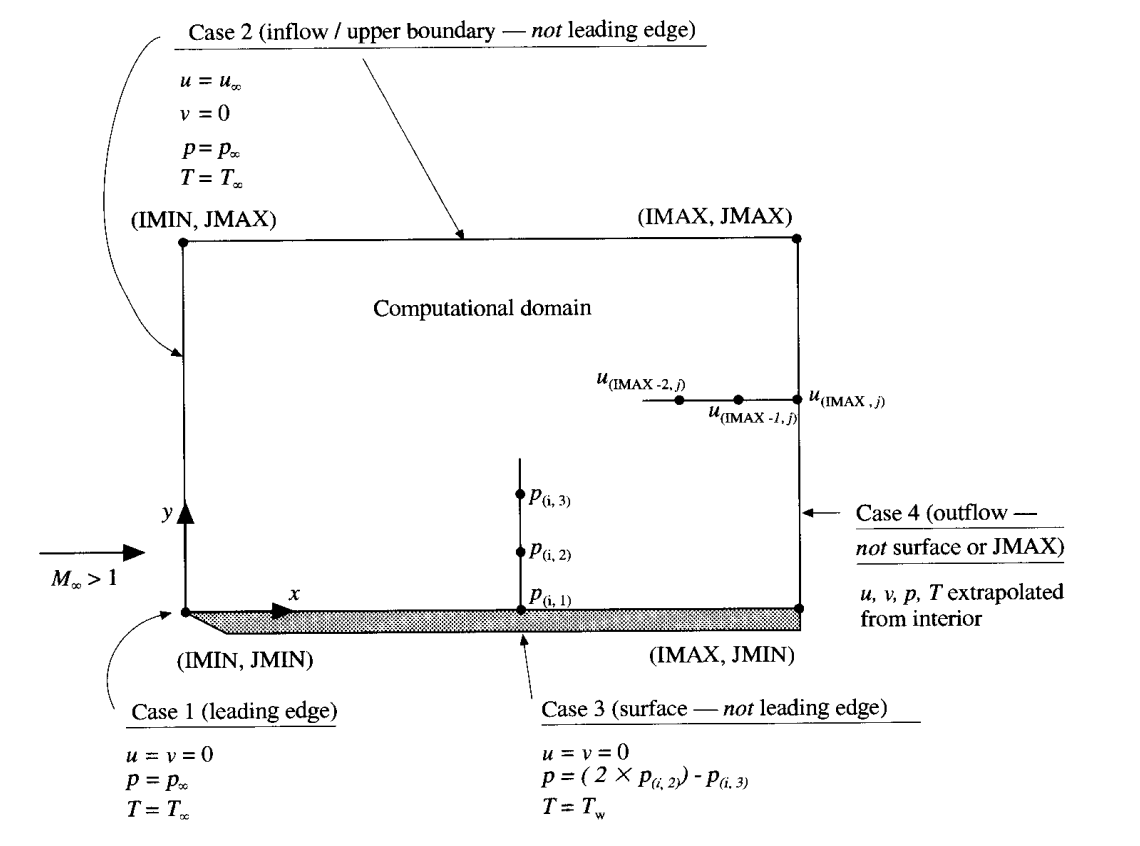
\includegraphics[scale=0.3]{supportingFiles/schematic_diagram.png}
    \caption{Schematic diagram along with boundary conditions for the
    present problem, taken from the book}
    \label{schematic_diagram}
\end{figure}


\section{Computation procedure}
\par The governing equations used in the work is given below.

\begin{align*}
    \frac{\partial U}{\partial t} + \frac{\partial E}{\partial x} + \frac{\partial F}{\partial y} = 0
\end{align*}

\begin{figure*}[!h]
   \centering
    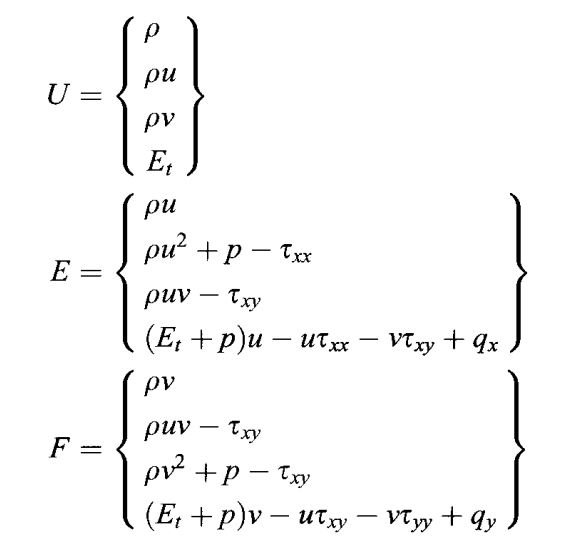
\includegraphics[scale=0.3]{supportingFiles/eqn_terms.png}
\end{figure*}

\par Apart from these, the additional equations used, that forms complete
Navier-Stokes equations are given below.
\begin{align*}
    \tau_{xy} &= \tau_{yx} = \mu \left( \frac{\partial u}{\partial y} + \frac{\partial v}{\partial x} \right) \\
    \tau_{xx} &= \lambda \left( \nabla . \vec{V}\right) + 2 \mu \frac{\partial u}{\partial x} \\
    \tau_{yy} &= \lambda \left( \nabla . \vec{V}\right) + 2 \mu \frac{\partial v}{\partial y} \\
    q_x &= -k \frac{\partial T}{\partial x} \\
    q_y &= -k \frac{\partial T}{\partial y} \\
    p &= \rho R T \\
    e &= C_v T\\
    \mu &= \mu_0\left(\frac{T}{T_0}\right)^{3/2} \frac{T_0+110}{T+110} \\
    k &= \frac{\mu C_p}{Pr}
\end{align*}

\par The equation used in computing the timestep using Courant-Friedrich-Lewy
condition is given below. The following equation is used to compute timestep
size for all internal grid points and the timestep for computation is chosen to
be the lowest of all multiplied with Courant number $K = 0.6$.
\begin{align*}
    \left(\Delta t_{CFL}\right)_{i,j} &= \left[\frac{|u_{i,j}|}{\Delta x} + \frac{|v_{i,j}|}{\Delta y}+ \sqrt{\gamma R T_{i,j}}\sqrt{\frac{1}{\Delta x^2} + \frac{1}{\Delta y^2}} + 2\nu_{i,j} \left(\frac{1}{\Delta x^2} + \frac{1}{\Delta y^2}\right)\right]^{-1} \\
    \Delta t &= K \times min\left(\Delta t_{CFL}\right)
\end{align*}

\par The algorithm followed for the computation is given below.
\begin{enumerate}
    \item The program is setup with required variables. The flow field variables
        such as temperature and pressure were initialized to free-stream values.
    \item The boundary conditions are applied, as indicated in the \Cref{schematic_diagram}.
    \item The conservative variables, U's, were computed from the primitive flow
        field variables. And the computation timestep is computed based on the
        flow field variables.
    \item The shear stresses and heat flux were computed using the derivatives
        of velocity that were computed from the current velocity fields.
    \item Then the conservative variables, E's and F's were computed from the
        primitive, shear stresses and heat flux variables.
    \item For the predictor step, the derivatives of E and F were computed using
        forward differencing and U derivatives were computed acoordingly.
    \item Then the predicted U values were computed and used to compute
        predicted primitive variables, then boundary conditions were applied
        and then the values were used to compute E's and Fs for the corrector
        step.
    \item The U derivatives of corrector step were computed from E and F derivatives
        and then the average of U derivatives from predictor and corrector steps
        were used to compute U values of next timestep.
    \item The primitive variables for next timestep is computed from the new
        U values and the boundary conditions were imposed, then the process
        is repeated from step 3 till convergence.
    \item Convergence is confirmed when the change in density values between
        each timestep is to be less than 1e-8.
\end{enumerate}

\section{Computation results}
\par The Fortran code is made in a modular way, such that any further modifications
and enhancements can be easily implemented. The converged solution is written
as a csv file from the Fortran code and the csv file is loaded into ParaView
for visualization. The contours obtained for the present case is shown in
\Cref{results_Tc}, this case is with constant wall temperature set to free-stream
temperature value.

\begin{figure}[!htb]
    \centering
    \begin{subfigure}{0.45\textwidth}
        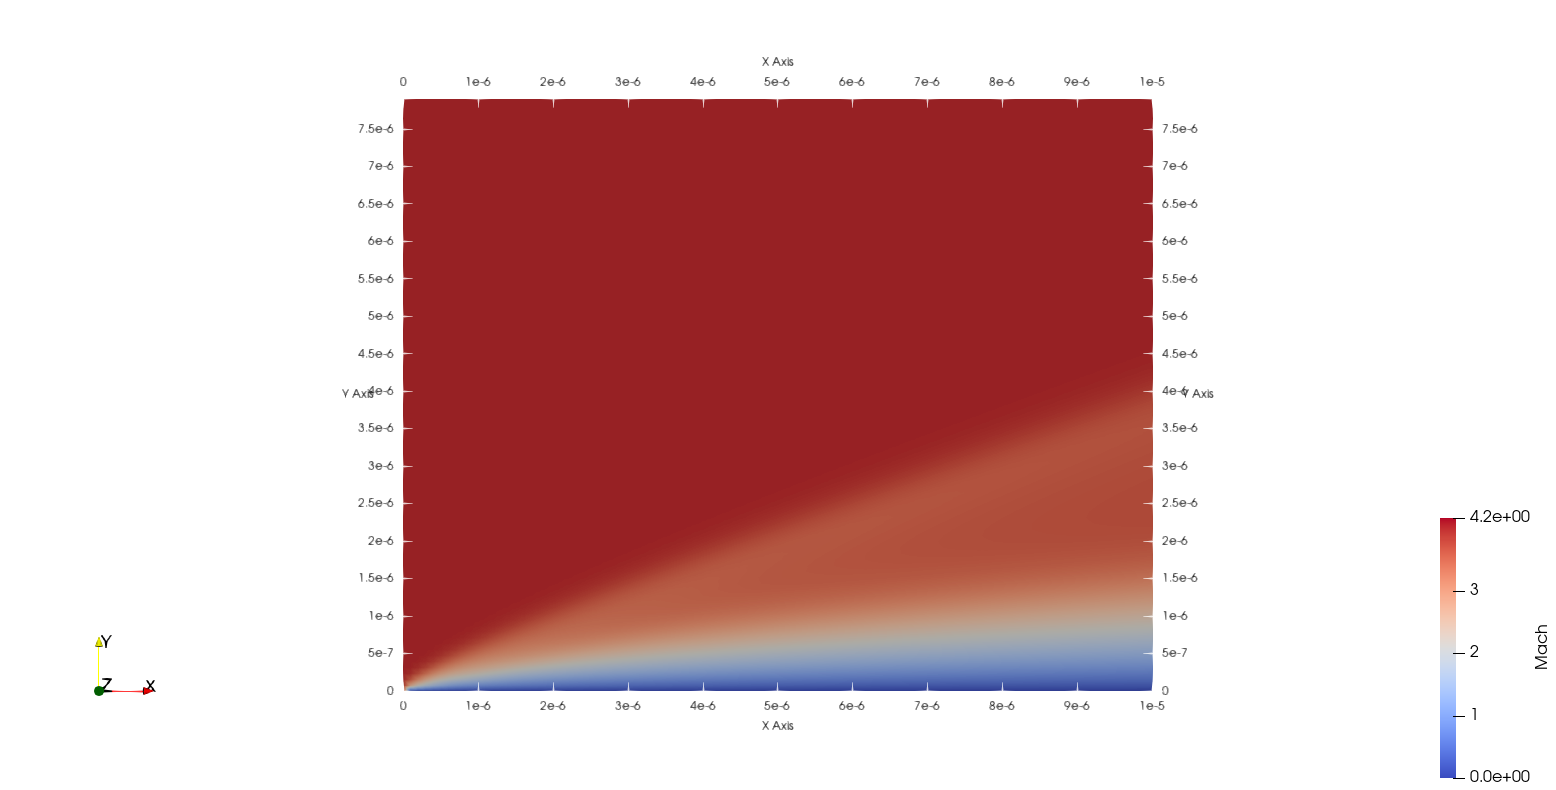
\includegraphics[width=\textwidth]{supportingFiles/solution_files_flatplate_constant_Twall/mach.png}
        \caption{Mach number contour}
    \end{subfigure}
    \hfill
    \begin{subfigure}{0.45\textwidth}
        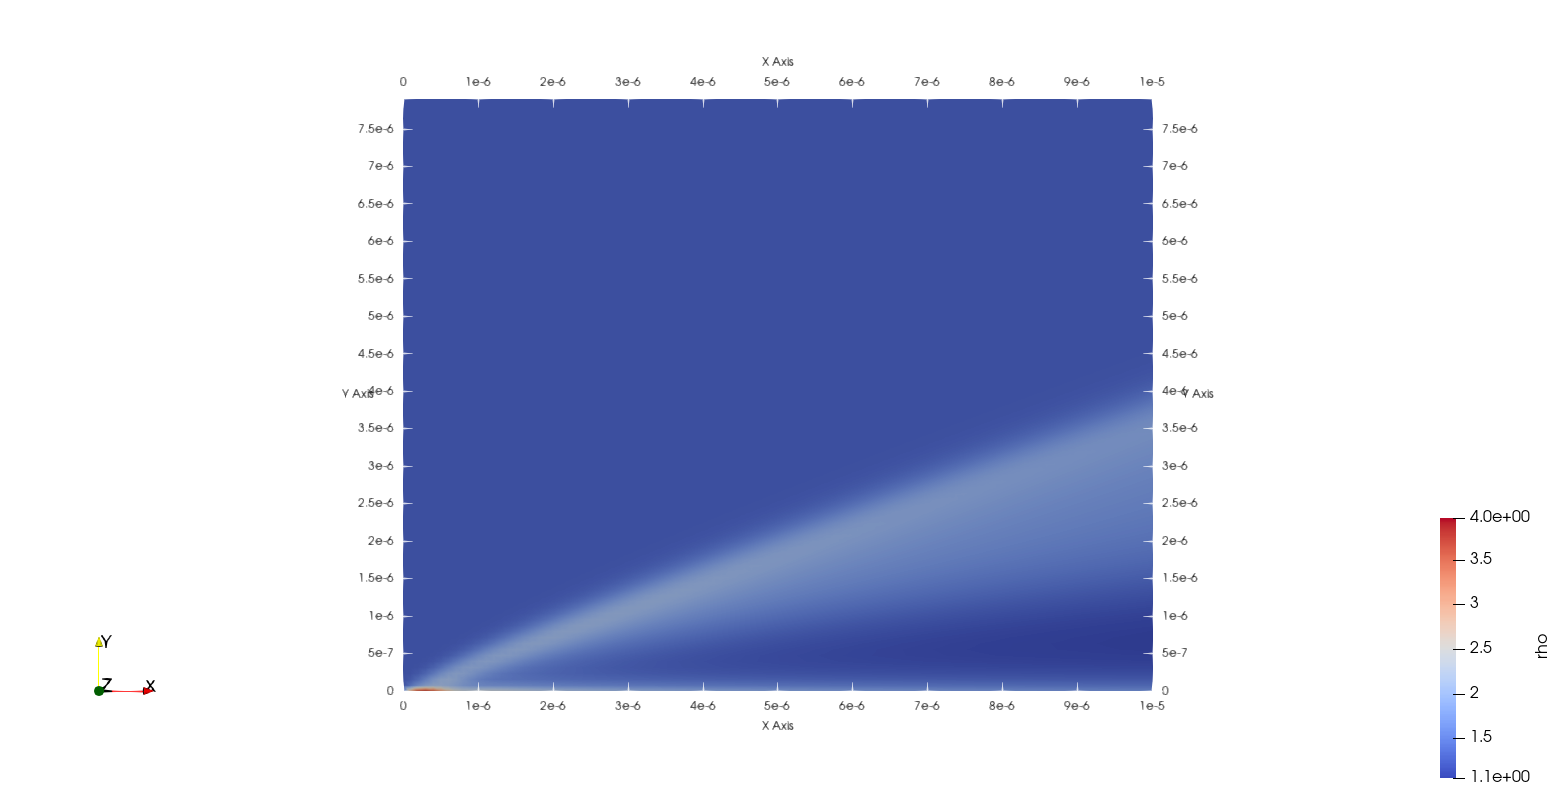
\includegraphics[width=\textwidth]{supportingFiles/solution_files_flatplate_constant_Twall/density.png}
        \caption{density contour}
    \end{subfigure}
    \hfill
    \begin{subfigure}{0.45\textwidth}
        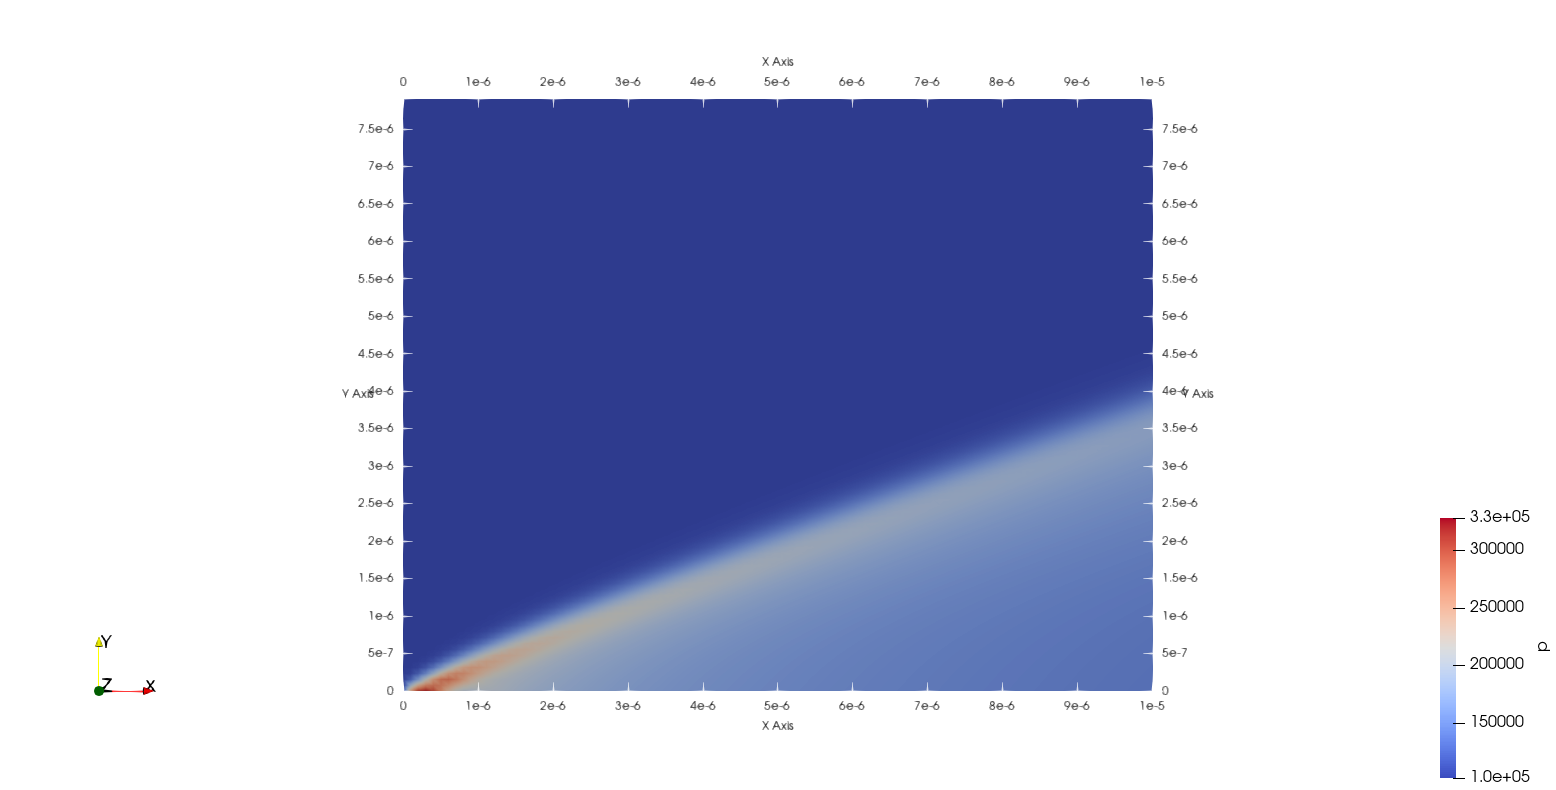
\includegraphics[width=\textwidth]{supportingFiles/solution_files_flatplate_constant_Twall/pressure.png}
        \caption{pressure contour}
    \end{subfigure}
    \hfill
    \begin{subfigure}{0.45\textwidth}
        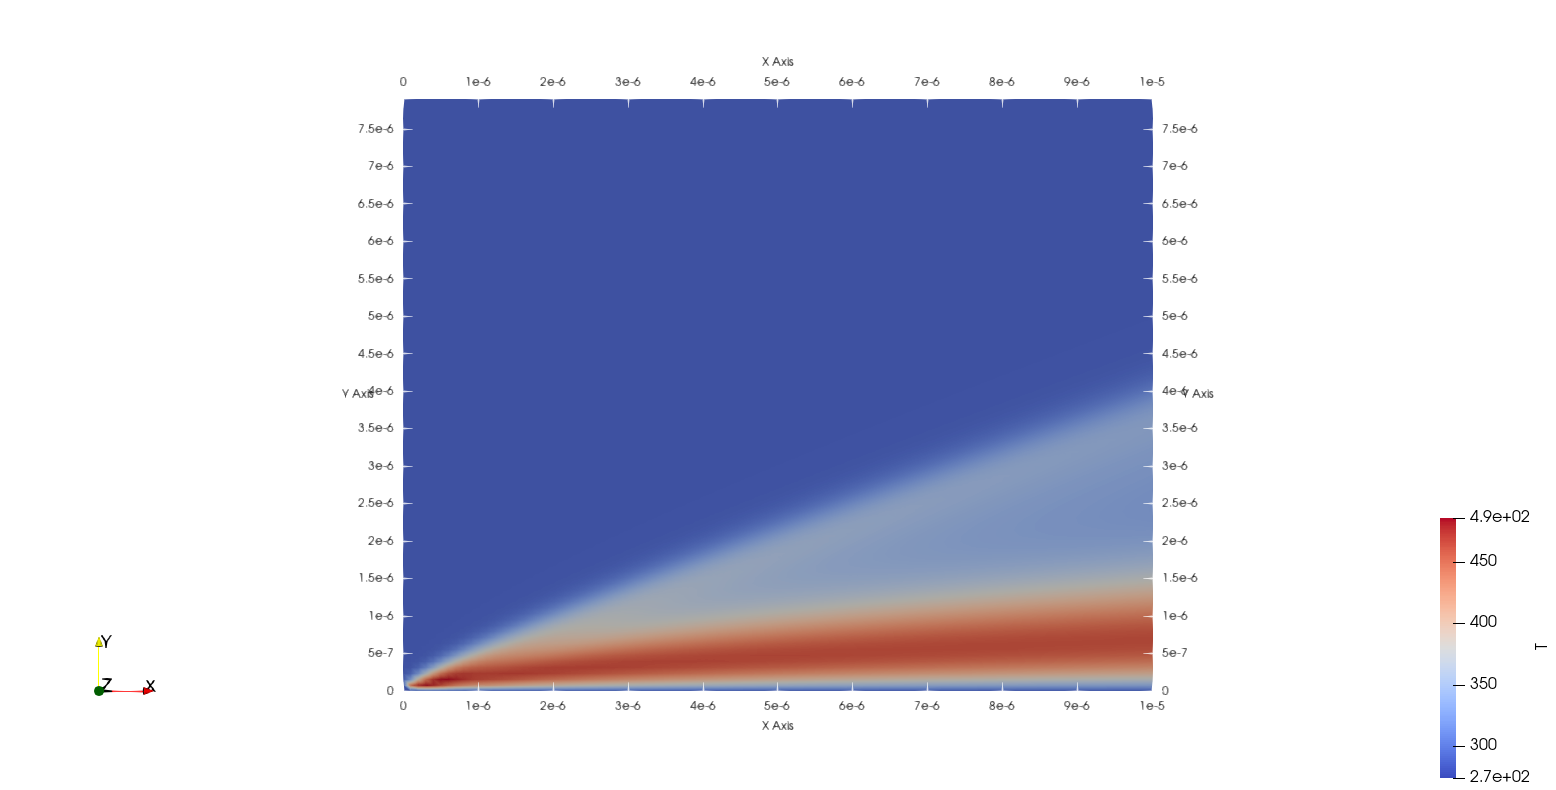
\includegraphics[width=\textwidth]{supportingFiles/solution_files_flatplate_constant_Twall/temperature.png}
        \caption{temperature contour}
    \end{subfigure}
    \hfill
    \begin{subfigure}{0.45\textwidth}
        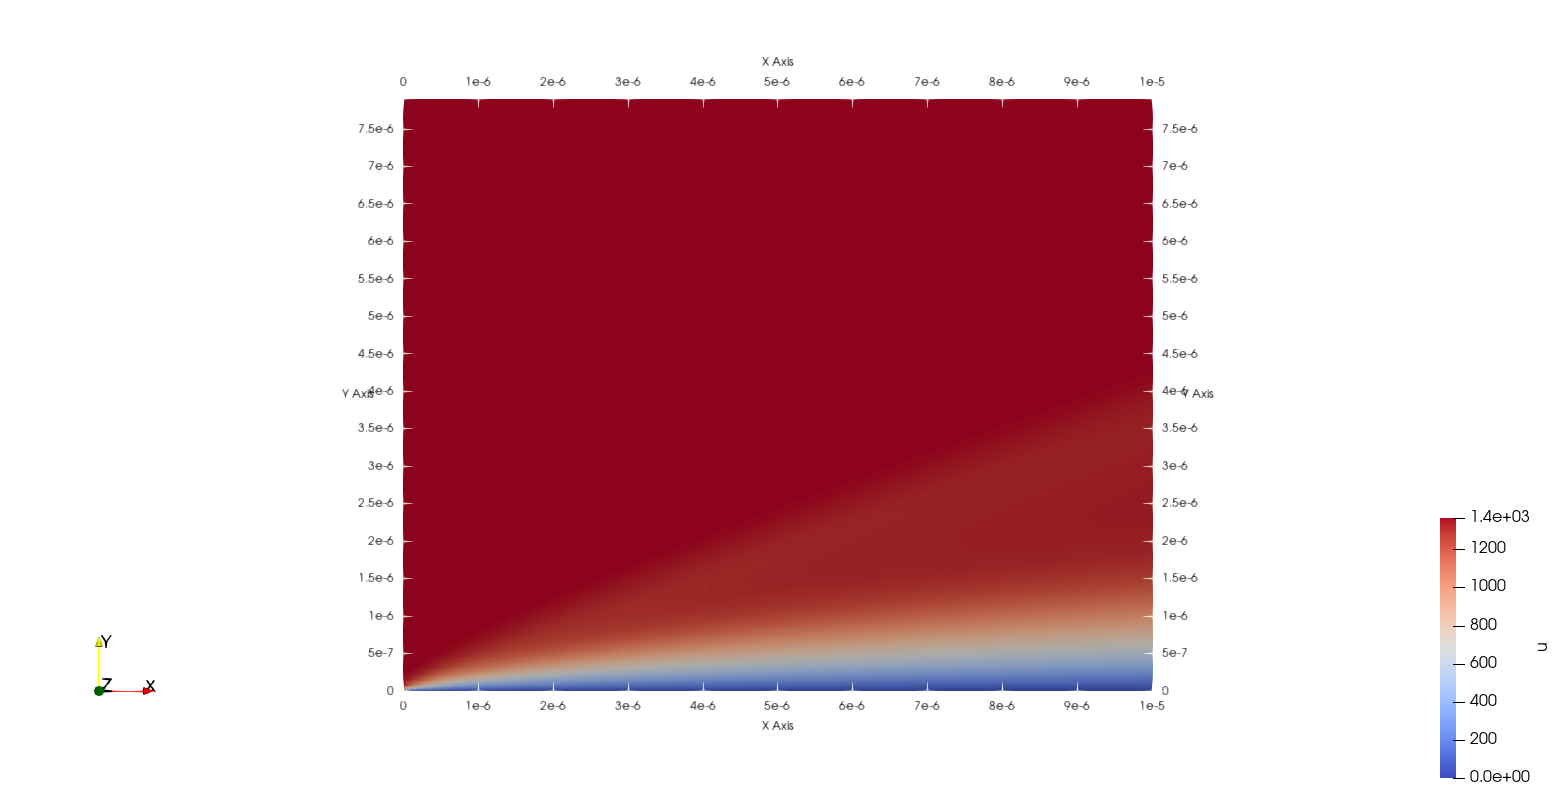
\includegraphics[width=\textwidth]{supportingFiles/solution_files_flatplate_constant_Twall/u_velocity.png}
        \caption{x-velocity contour}
    \end{subfigure}
    \hfill
    \begin{subfigure}{0.45\textwidth}
        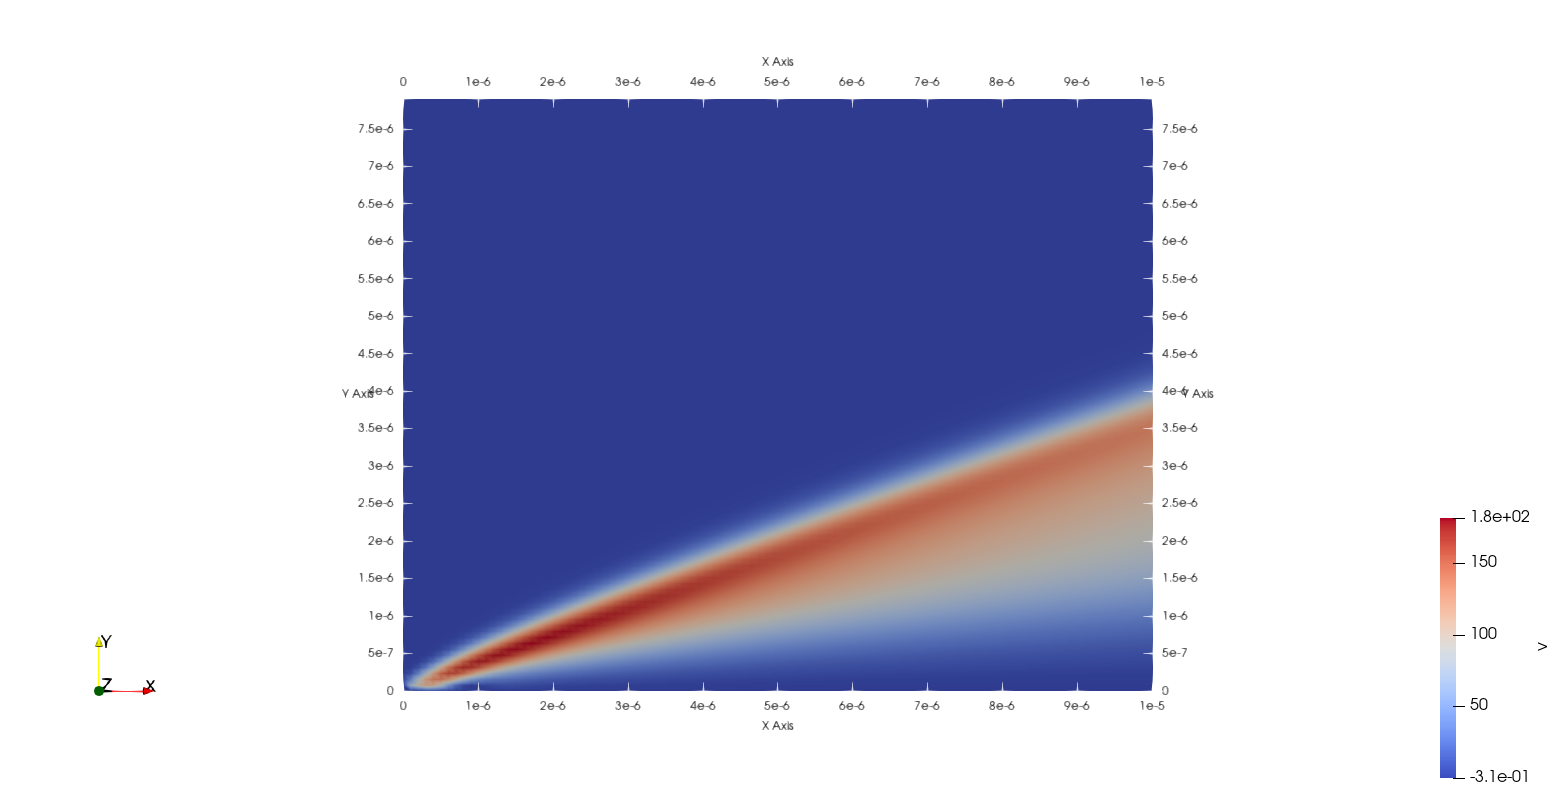
\includegraphics[width=\textwidth]{supportingFiles/solution_files_flatplate_constant_Twall/v_velocity.png}
        \caption{y-velocity contour}
    \end{subfigure}
    \caption{Computation results of case with constant wall temperature, set to free-stream temperature}
    \label{results_Tc}
\end{figure}

\par Further, another case with adiabatic wall temperature was computed, those results are given in
\Cref{results_Wa}

\begin{figure}[!htb]
    \centering
    \begin{subfigure}{0.45\textwidth}
        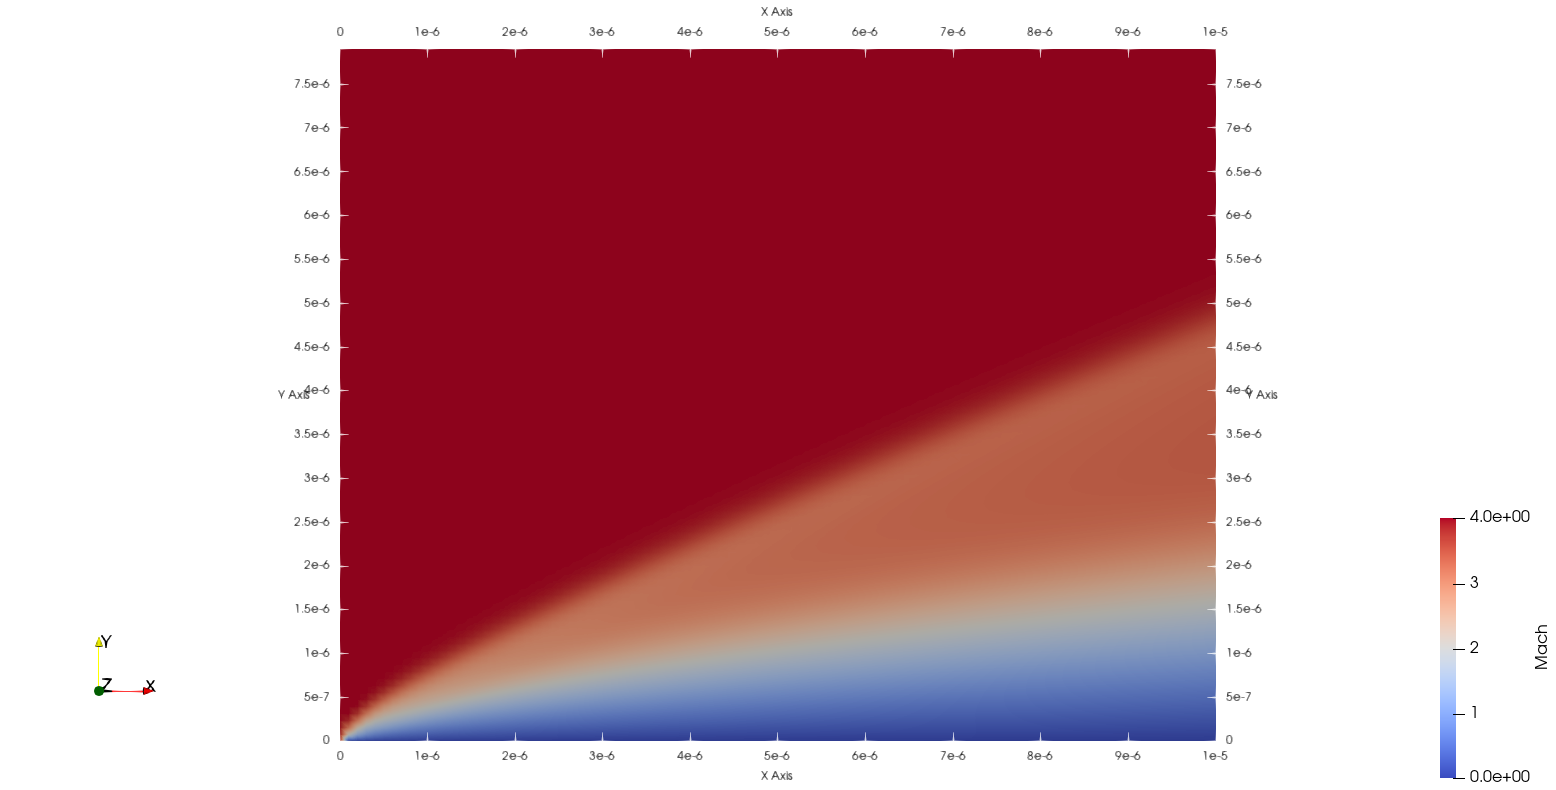
\includegraphics[width=\textwidth]{supportingFiles/solution_files_flatplate_adiabaticWall/mach.png}
        \caption{Mach number contour}
    \end{subfigure}
    \hfill
    \begin{subfigure}{0.45\textwidth}
        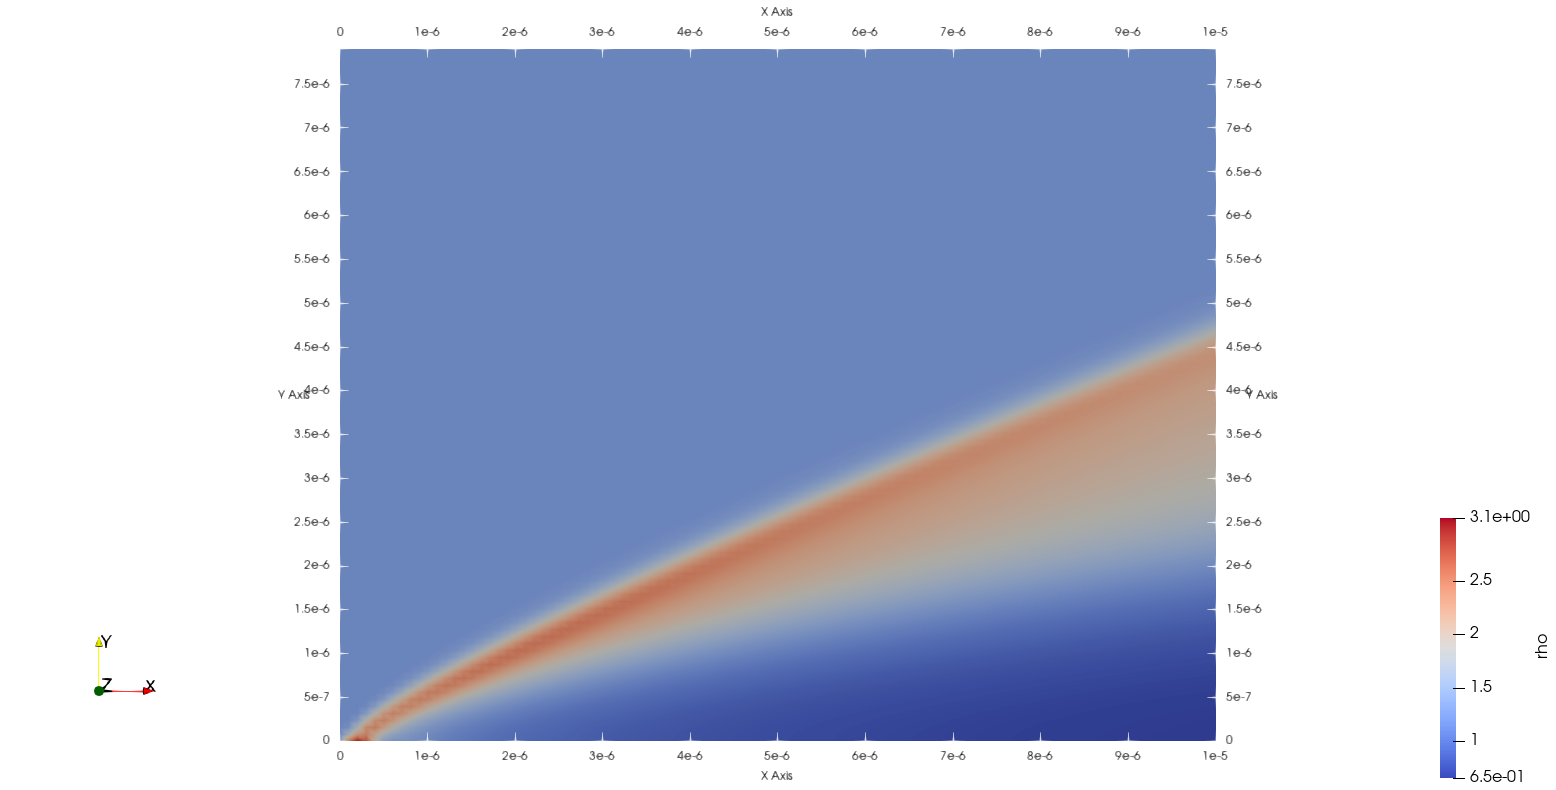
\includegraphics[width=\textwidth]{supportingFiles/solution_files_flatplate_adiabaticWall/density.png}
        \caption{density contour}
    \end{subfigure}
    \hfill
    \begin{subfigure}{0.45\textwidth}
        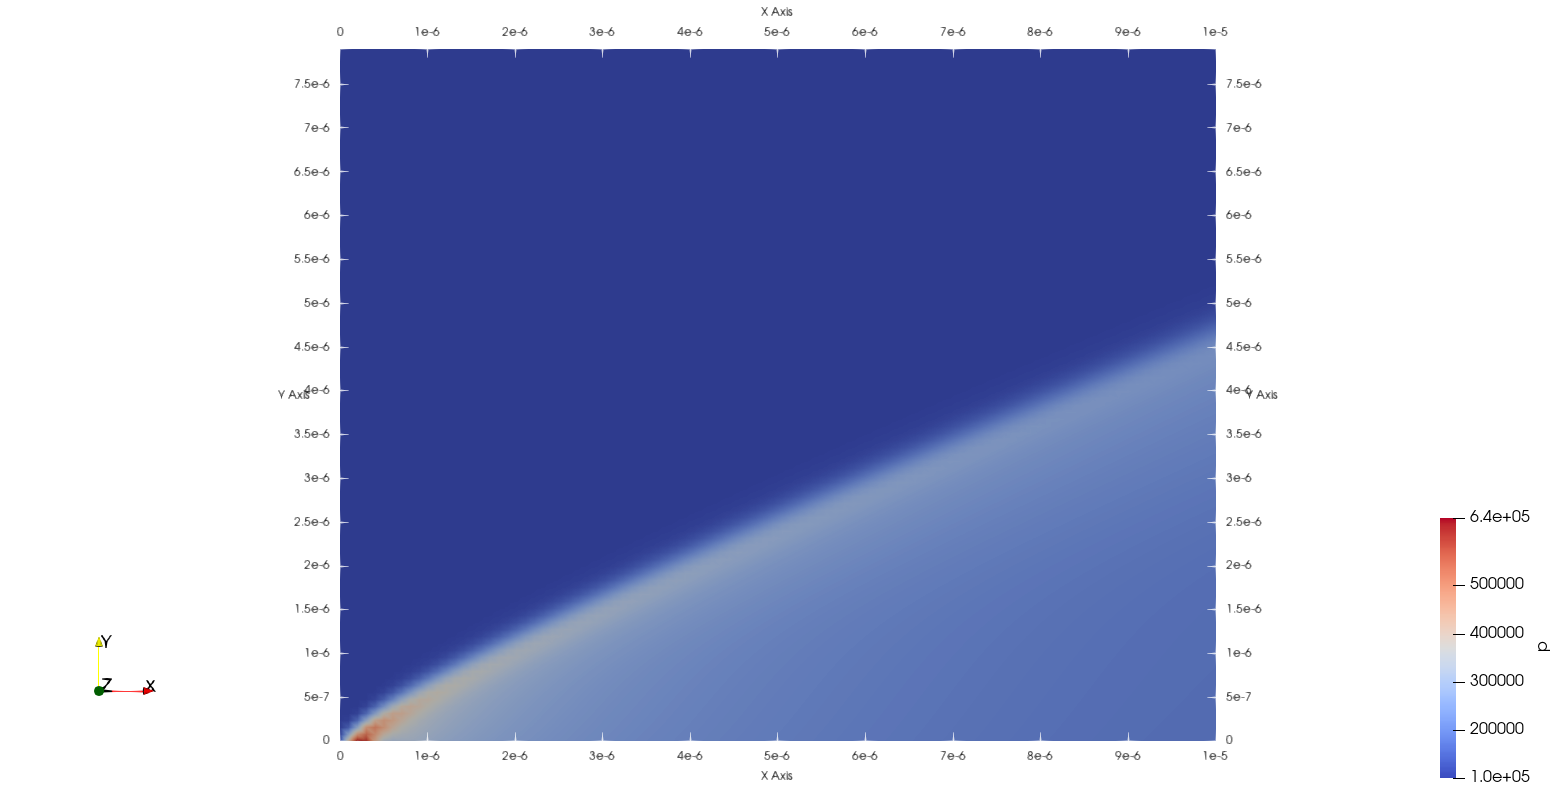
\includegraphics[width=\textwidth]{supportingFiles/solution_files_flatplate_adiabaticWall/pressure.png}
        \caption{pressure contour}
    \end{subfigure}
    \hfill
    \begin{subfigure}{0.45\textwidth}
        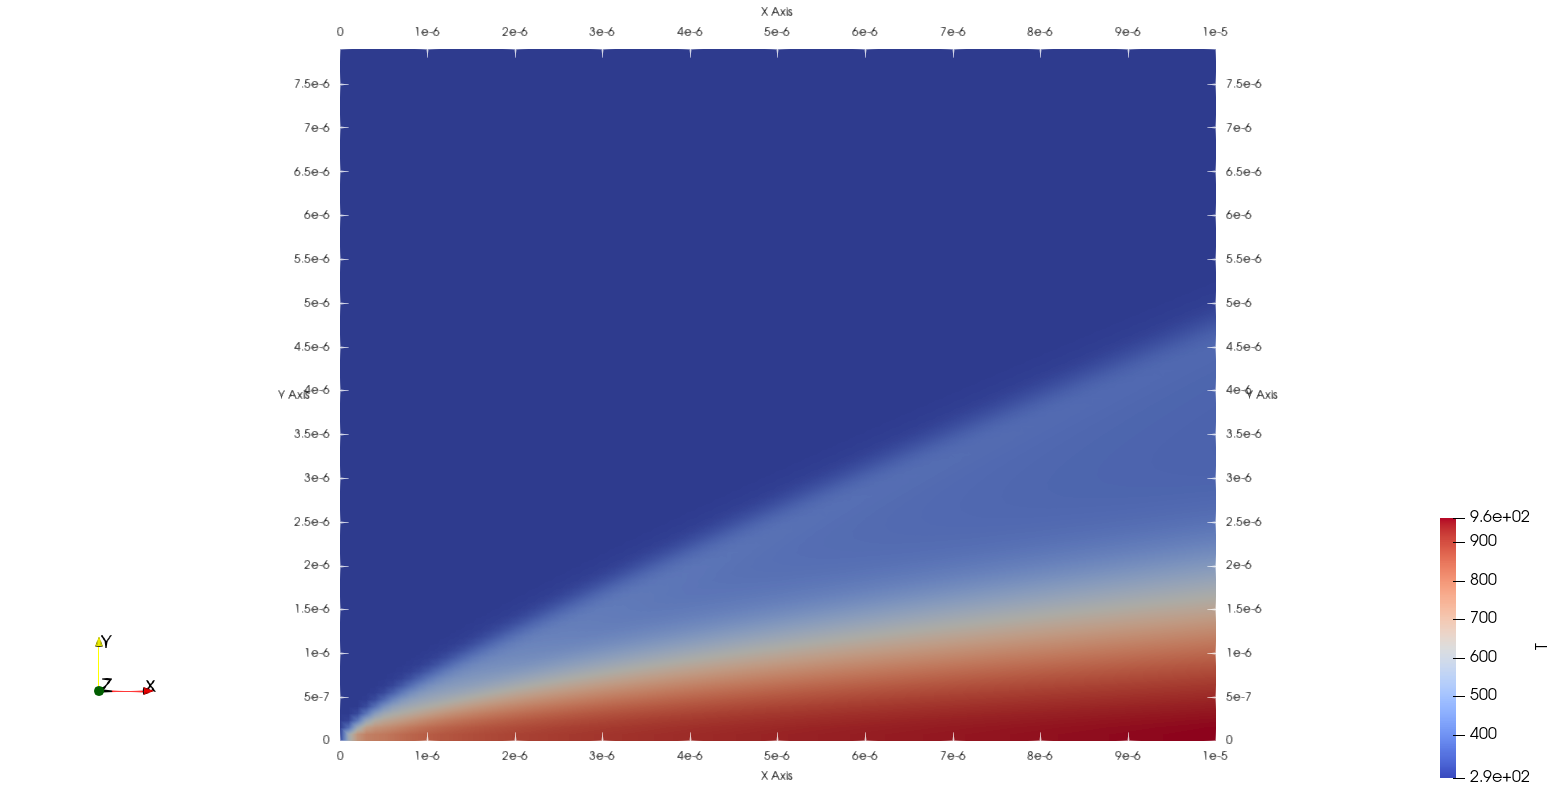
\includegraphics[width=\textwidth]{supportingFiles/solution_files_flatplate_adiabaticWall/temperature.png}
        \caption{temperature contour}
    \end{subfigure}
    \hfill
    \begin{subfigure}{0.45\textwidth}
        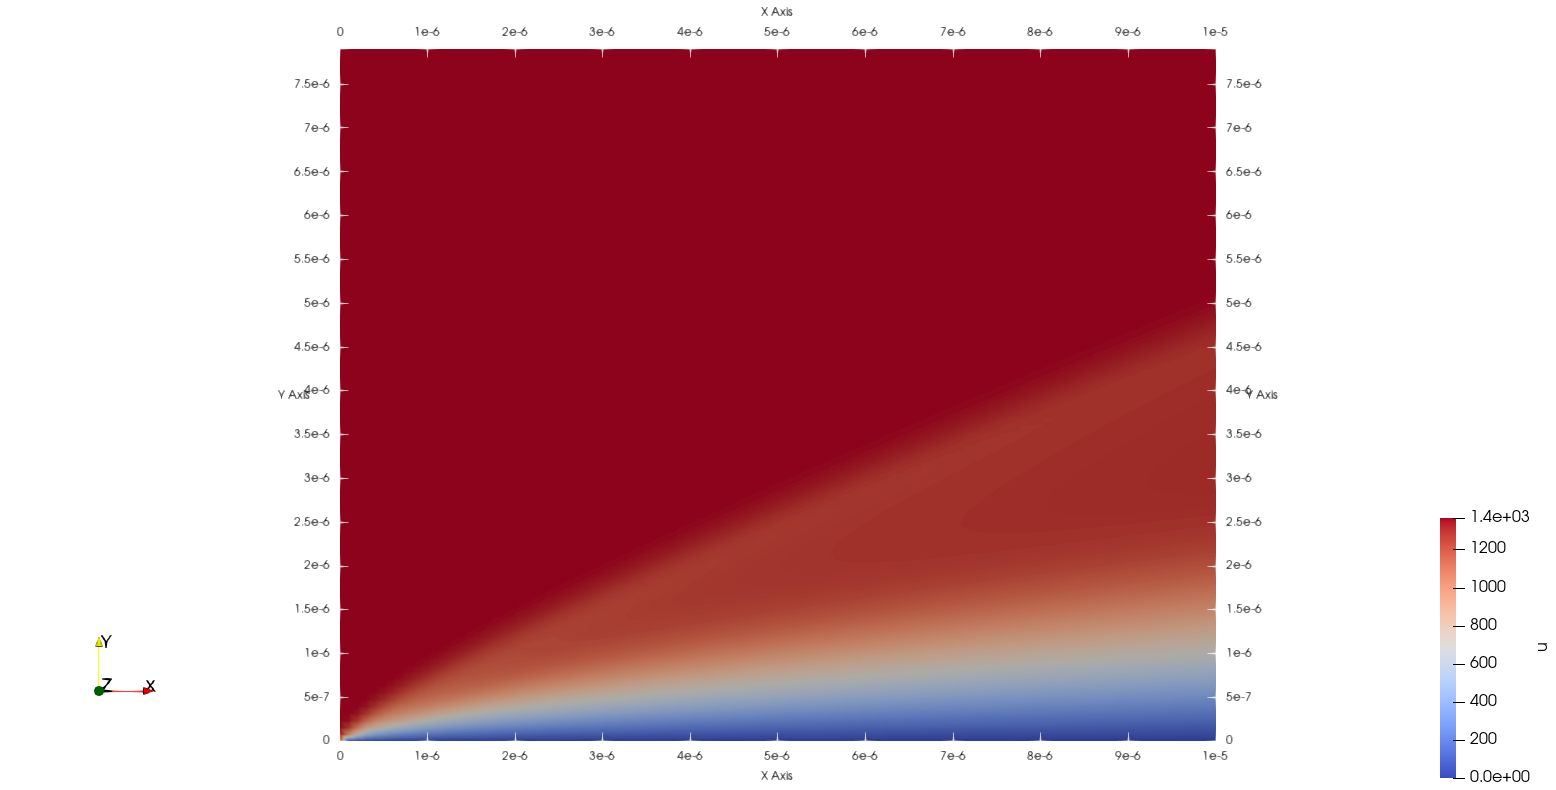
\includegraphics[width=\textwidth]{supportingFiles/solution_files_flatplate_adiabaticWall/u_velocity.png}
        \caption{x-velocity contour}
    \end{subfigure}
    \hfill
    \begin{subfigure}{0.45\textwidth}
        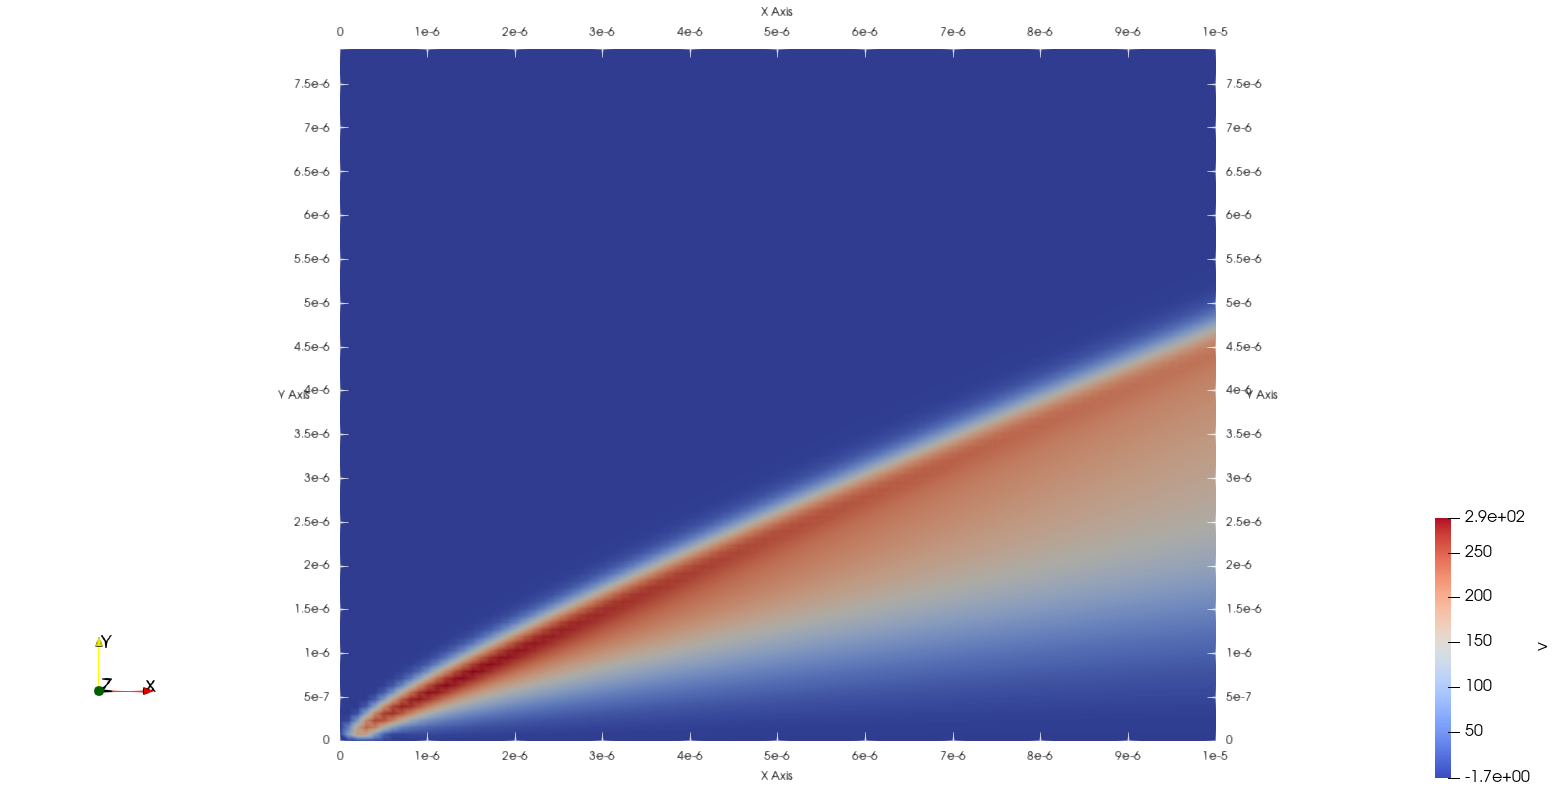
\includegraphics[width=\textwidth]{supportingFiles/solution_files_flatplate_adiabaticWall/v_velocity.png}
        \caption{y-velocity contour}
    \end{subfigure}
    \caption{Computation results of case with adiabatic wall temperature}
    \label{results_Wa}
\end{figure}

\par And, another case with flow entering with an angle of -10 degrees with x-axis i.e.
flowing downwards with 10 degrees with the horizontal, is made by modifying
boundary conditions to simulate the supersonic flow over a wedge inclined at 10 degrees with
flow direction. The results obtained in this case is validated by comparing the
average downstream Mach number with the theorectical value. The results are
given in \Cref{results_os}.

\par Clear contours for all the cases were present with the code in the github
repository.

\begin{figure}[!htb]
    \centering
    \begin{subfigure}{0.75\textwidth}
        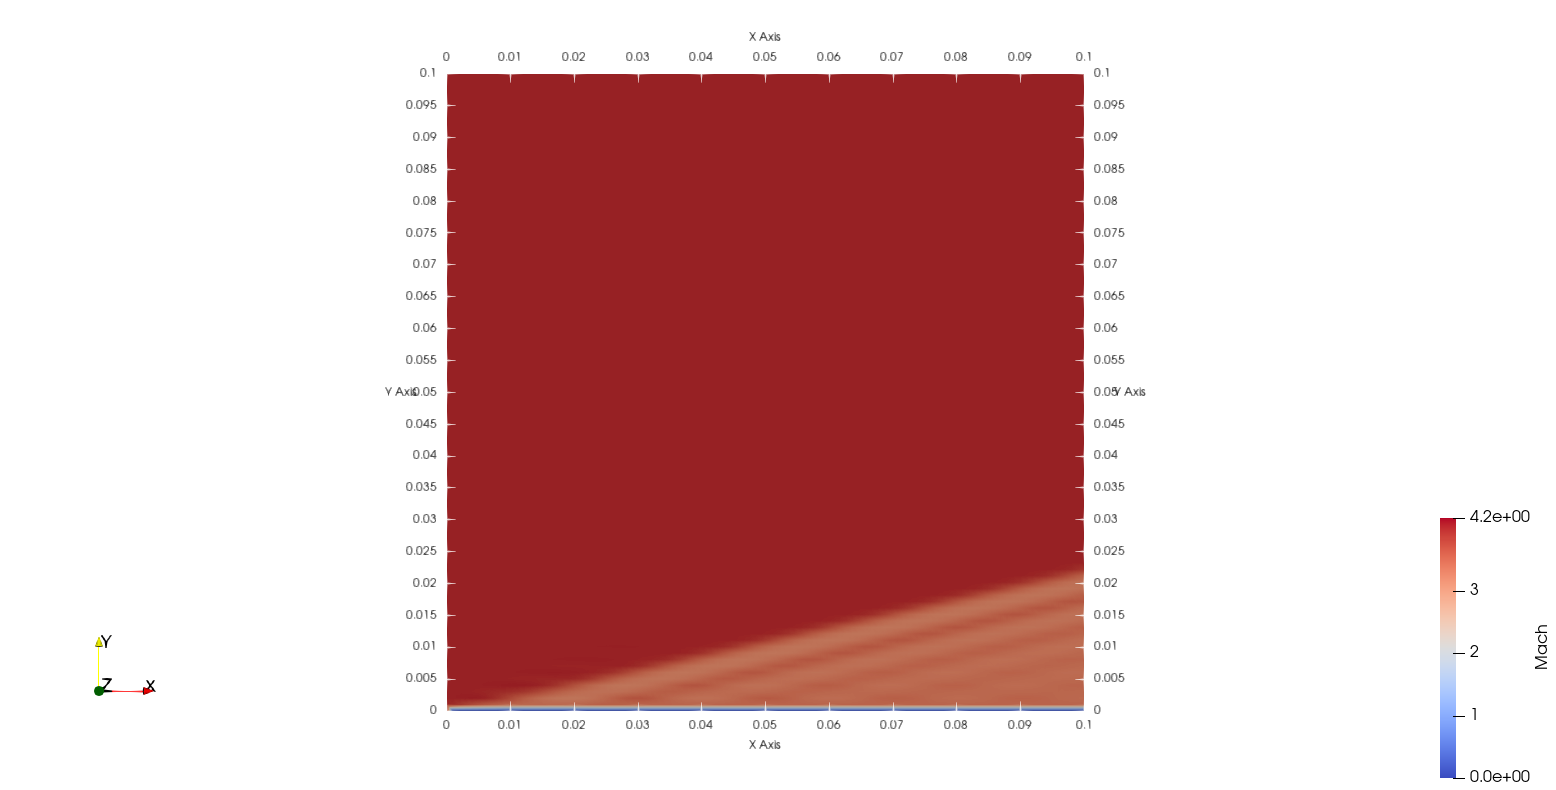
\includegraphics[width=\textwidth]{supportingFiles/solution_files_obliqueShock/oblique_shock_10_mach.png}
        \caption{Mach number contour}
    \end{subfigure}
    \hfill
    \begin{subfigure}{0.75\textwidth}
        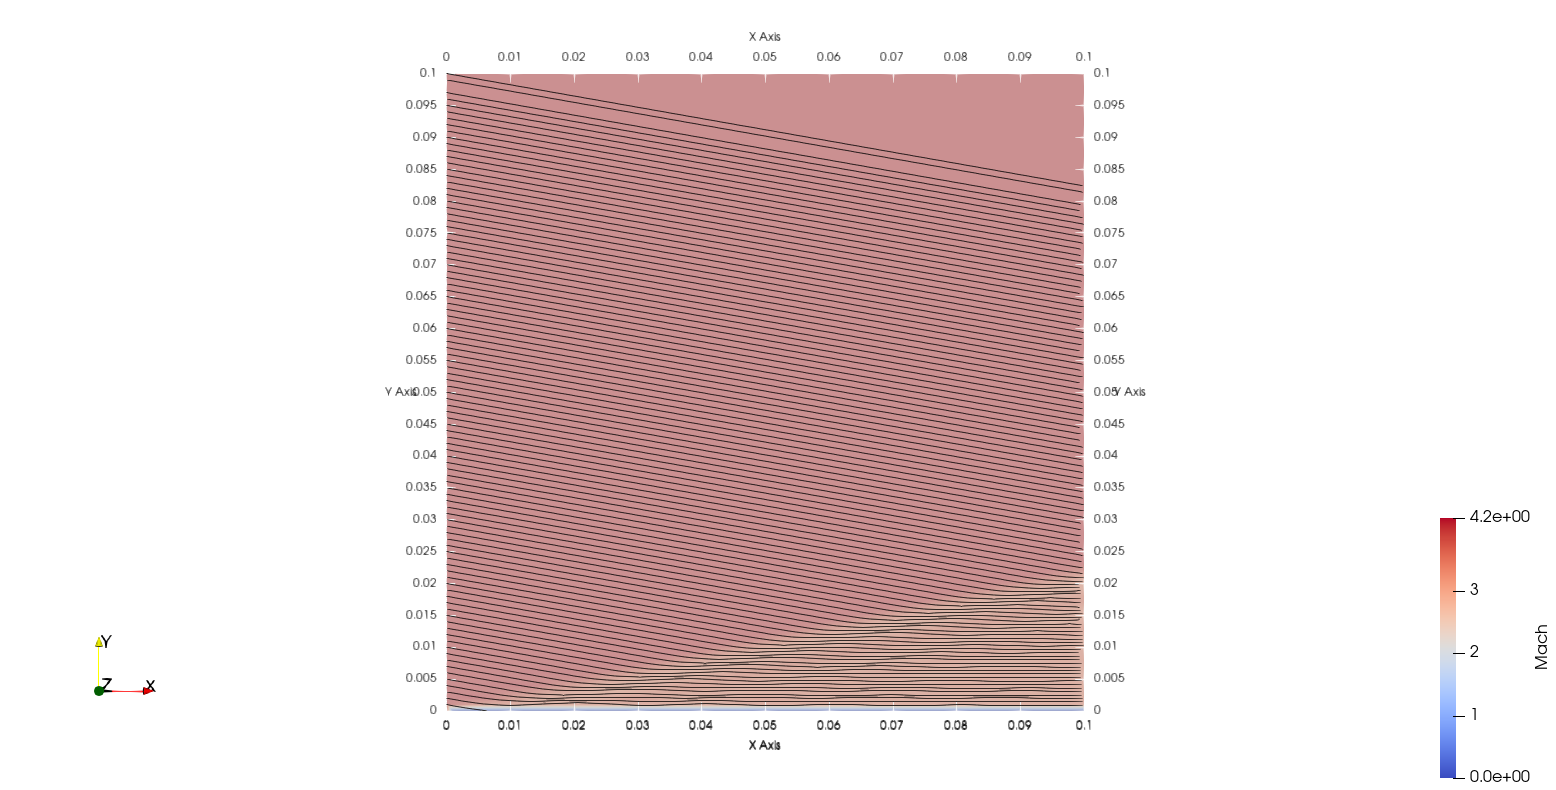
\includegraphics[width=\textwidth]{supportingFiles/solution_files_obliqueShock/streamlines_obliqueshock.png}
        \caption{streamline pattern showing the flow direction}
    \end{subfigure}
    \caption{Computation results of case simulating oblique shock}
    \label{results_os}
\end{figure}


\section{Conclusion and Future works}
The laminar viscous supersonic flow over flat plate were numerically computed
using Finite difference method and full Navier-Stokes equations. The Fortran
code is made modular so that any further modifications and enhancements can be
implemented. The following enhancements are planned to make.
\begin{itemize}
    \item transforming 2D version of code to 3D.
    \item adding advanced solvers and turbulence models to the code.
    \item implementing grid transformations, so that curvilinear grids
        can also be solved using this code.
    \item solving capability with dynamic meshing.
\end{itemize}

\par The Fortran code, along with this documentation can be found in the
Github repository at \url{https://github.com/Ramkumar47/ComputationalCodes/05_supersonicFlow_over_flatPlate/}

% \section{Question}

\begin{figure*}[!h]
    \center
    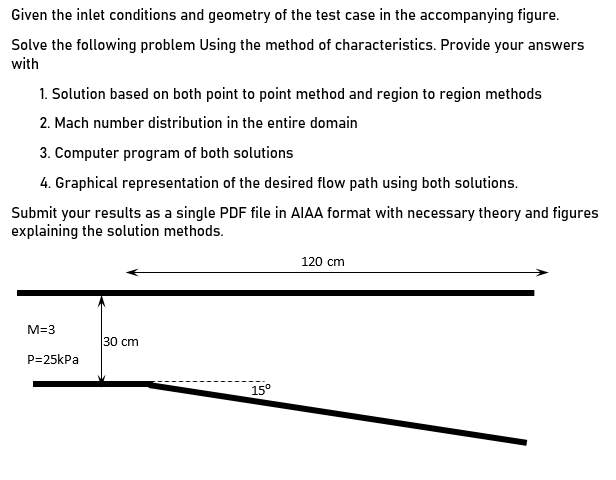
\includegraphics[scale=0.5]{results/question.png}
\end{figure*}

\textbf{SOLUTION:}\\

\par Given data
\begin{align*}
    M_1 &= 3.0 \\
    h &= 0.3 \ m \\
    L &= 1.2 \ m \\
    P_1 &= 25 \ kPa
\end{align*}

\par The solution algorithm followed for this problem is given below.\\

\par The number of characteristic nodes N, in the inlet plane is first chosen. The
value chosen for this problem is 100. An example layout of Characteristic lines
with N = 6, in the expansion flow domain of deflection angle $2^{\circ}$ is given in
\Cref{domain_layout}.But, the actual problem with $15^{\circ}$ deflection angle
requies N = 100 in order to accurately capture the expansion flow field. \\

\begin{figure}
   \center
    \includegraphics[scale=0.9]{results/expansion_corner_trial/char_map.png}
    \caption{Coarse characteristic points layout on the $2^{\circ}$ expansion corner}
    \label{domain_layout}
\end{figure}

\par Then the total number of characteristic nodes that will appear after all
interactions is computed using the equation below. Here, $n_{wall}$ is the number
of wall bounces requried as it is the one that controls the length of the
computation domain in this case. \\
\begin{align*}
    N_{total} = n_{wall} (2 N - 1) + N
\end{align*}

\par After this, a list of numbers indicating the characteristic points were
generated linearly similar to the one shown in \Cref{domain_layout} and the
points on both top and bottom wall is identified using the below equations
and were grouped for ease of computation.
\begin{align*}
    bottom\ wall: n_b = n_{b,prev} + (2N -1) \\
    top\ wall: n_b = n_{b,prev} + (N -1) \\
\end{align*}

\par Then a table, with the list of dependence upstream characteristic points,
to each internal and boundary char.point is made, which will be used during
computations. The inlet condition is defined such that, the expansion function
values $\nu(M)$ at all inlet char.points is computed for the following specified
condition. And the values of $K_1$ and $K_2$ were computed using the relations
given.
\begin{align*}
    M_{inlet} &= 3.0  \\
    \theta_{inlet} &= 0.0 \\
    K_1 &= \nu + \theta \\
    K_2 &= \nu - \theta
\end{align*}

\par Then the computation is begun for internal points, where the values of
$\nu$ and $\theta$ were computed by taking the intersected $K_1$ and $K_2$
upstream values as shown below.
\begin{align*}
    \nu &= \frac{K_1 + K_2}{2} \\
    \theta &= \frac{K_1 - K_2}{2}
\end{align*}

\par At the wall points, only one upstream characteristics meet, but the
wall angle $\theta_{wall}$ is known, hence using the upstream characteristic
and wall angle values, the expansion function is computed as shown in the
example below.
\begin{align*}
    bottom\ wall: \nu &= K_1 - \theta \\
    top\ wall: \nu &= K_2 + \theta
\end{align*}

\par Then, the Mach numbers at each characteristic point were computed using
Prandtl-Meyer expansion function relation given below.
\begin{align*}
    \nu(M) = \sqrt{\frac{\gamma+1}{\gamma-1}}tan^{-1}\sqrt{\frac{\gamma-1}{\gamma+1}\left(M^2-1\right)} - tan^{-1}\sqrt{M^2-1}
\end{align*}

\par For computing the location of downstream char.point, the following equations
that determine the slope of line (with the assumption that the char. curves are
straight lines in short length) and the location of the point as shown in the
\Cref{slope_image}.
\begin{figure}
    \center
    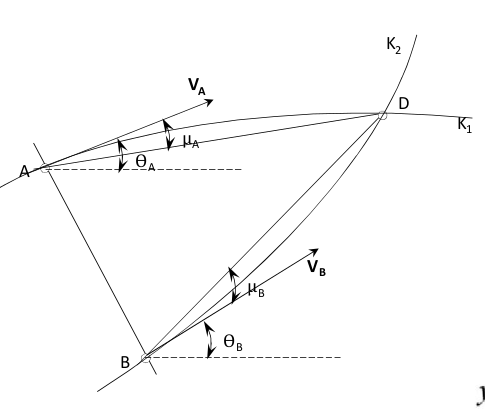
\includegraphics[scale=0.5]{results/slopeImage.png}
    \caption{reference image for the char. point position calculations}
    \label{slope_image}
\end{figure}


\begin{align*}
    \left(\frac{dy}{dx}\right)_A &= tan(\theta-\mu)_A \\
    \left(\frac{dy}{dx}\right)_B &= tan(\theta+\mu)_B \\
    S_1 &= \frac{tan(\theta-\mu)_A + tan(\theta-\mu)_B}{2} \\
    S_2 &= \frac{tan(\theta+\mu)_A + tan(\theta+\mu)_B}{2} \\
    y_D &=y_A + (x_D - x_A) S_1 \\
    y_D &=y_B + (x_D - x_B) S_2 \\
    x_D &= \frac{(S_2 x_B - S_1 x_A) + (y_A - y_B)}{S_2-S_1}
\end{align*}

\pagebreak
\textbf{Results:}

The Python code was developed for this computation and given in \Cref{appendixA}.
The contour of Mach number distribution and the characteristic points
obtained for this problem is given in \Cref{Mach_contour,char_output}, respectively. \\
\begin{figure}
    \center
    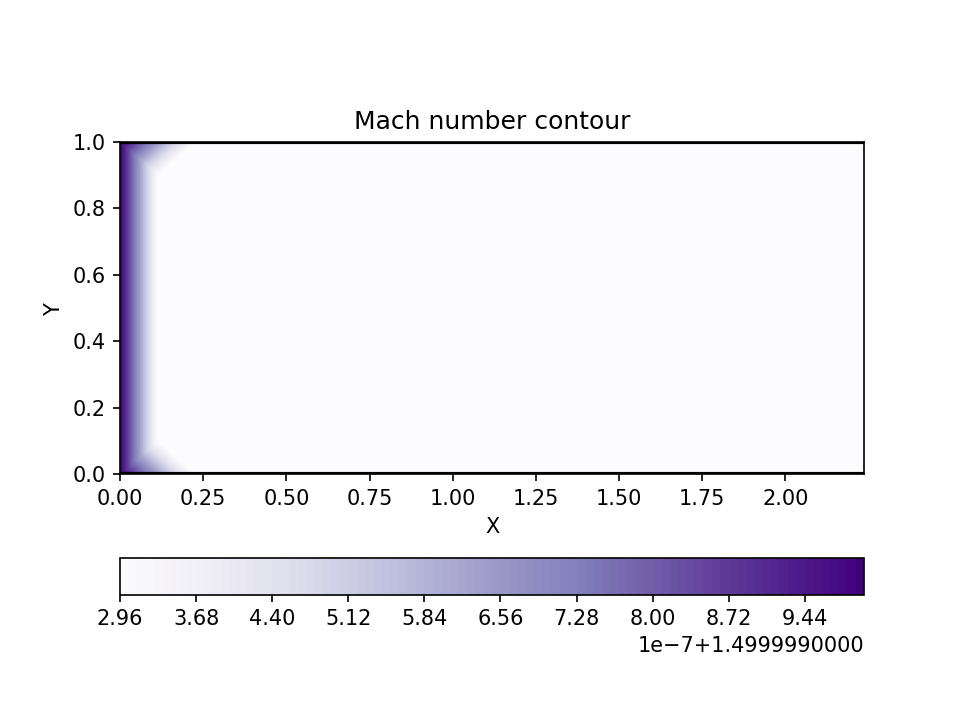
\includegraphics[scale=0.9]{results/expansion_corner/M_contour.png}
    \caption{Mach number contour output from computation}
    \label{Mach_contour}
\end{figure}

\begin{figure}
    \center
    \includegraphics[scale=0.9]{results/expansion_corner/char_map.png}
    \caption{characteristic points distribution (conjested due to 18k points for N = 100)}
    \label{char_output}
\end{figure}

\par Further, the Mach number of downstream section after expansion, obtained
from the computation is compared with the theoretical value obtained
from \cite{ref_1}. The following gives the values obtained and they found to
be in agreement with the theory.
\begin{align*}
    M_{2,computation} &= 3.92329 \\
    M_{2,theory} &= 3.923
\end{align*}

\pagebreak


% \begin{thebibliography}{2}
%     \bibitem{ref_1} Online Prandtl-Meyer expansion flow calculator; https://www.omnicalculator.com/physics/prandtl-meyer-expansion
%     \bibitem{ref_2} Michel A. Saad; Compressible fluid flow
%
% \end{thebibliography}

% \pagebreak

% \begin{appendices}
%     \section{Appendix - Python code for blockMeshDict}\label{appendixA}
%     This section contains the \emph{Python} code developed for the generation
%     of blockMeshDict file with specific flow deflection angle of shock-generator.
%
%     \lstinputlisting[language=Python]{supportingFiles/script_blockDefinition.py}
%
% \end{appendices}

\par
\center{**********}

\end{document}
